\documentclass[10pt,a4paper,leqno]{article}
\usepackage{CJKutf8}
\usepackage[utf8]{inputenc}
\usepackage[T1]{fontenc}
\usepackage{amsmath,esint}
\usepackage{amsfonts}
\usepackage{amssymb}
\usepackage{xcolor}
\usepackage{mathrsfs}
\usepackage{makeidx}
\usepackage{graphicx}
\usepackage{float}
\usepackage{gensymb}
\usepackage{textcomp}
\usepackage{longtable}
\usepackage{ifpdf}
\usepackage{tikz}                            
\usetikzlibrary{shapes,arrows}               
%\usepackage{tgothic}
\ifpdf
\usepackage[breaklinks,hidelinks]{hyperref}
\else 
\usepackage{url}
\fi
\newcommand*\VF[1]{\mathbf{#1}}
\newcommand*\dif{\mathop{}\!\mathrm{d}}
\author{CBCO}
\title{eNotes: The Conic Section}
\date{}
\begin{document}
\maketitle

\noindent \numberwithin{equation}{section} % This line resets equation numbering when starting a new section. 
\renewcommand{\theequation}{\thesection.\arabic{equation}}  
%\renewcommand{\theequation}{Eq. \thesection.\arabic{equation}} % This line ads Eq.
 \par \ \par\noindent \numberwithin{figure}{section}
% \renewcommand{	heequation}{Eq. 	hesection.rabic{equation}}
 \par \ \par\noindent \begin{CJK*}{UTF8}{gbsn}
 \par \ \par\noindent \section{Introduction }
 \par \ \par\noindent A conic section is an intersection of a cone with a plane.
 \par \ \par\noindent In Figure 1.1, the cones were plotted with two different methods.
 \par \ \par\begin{figure}[H]
\centering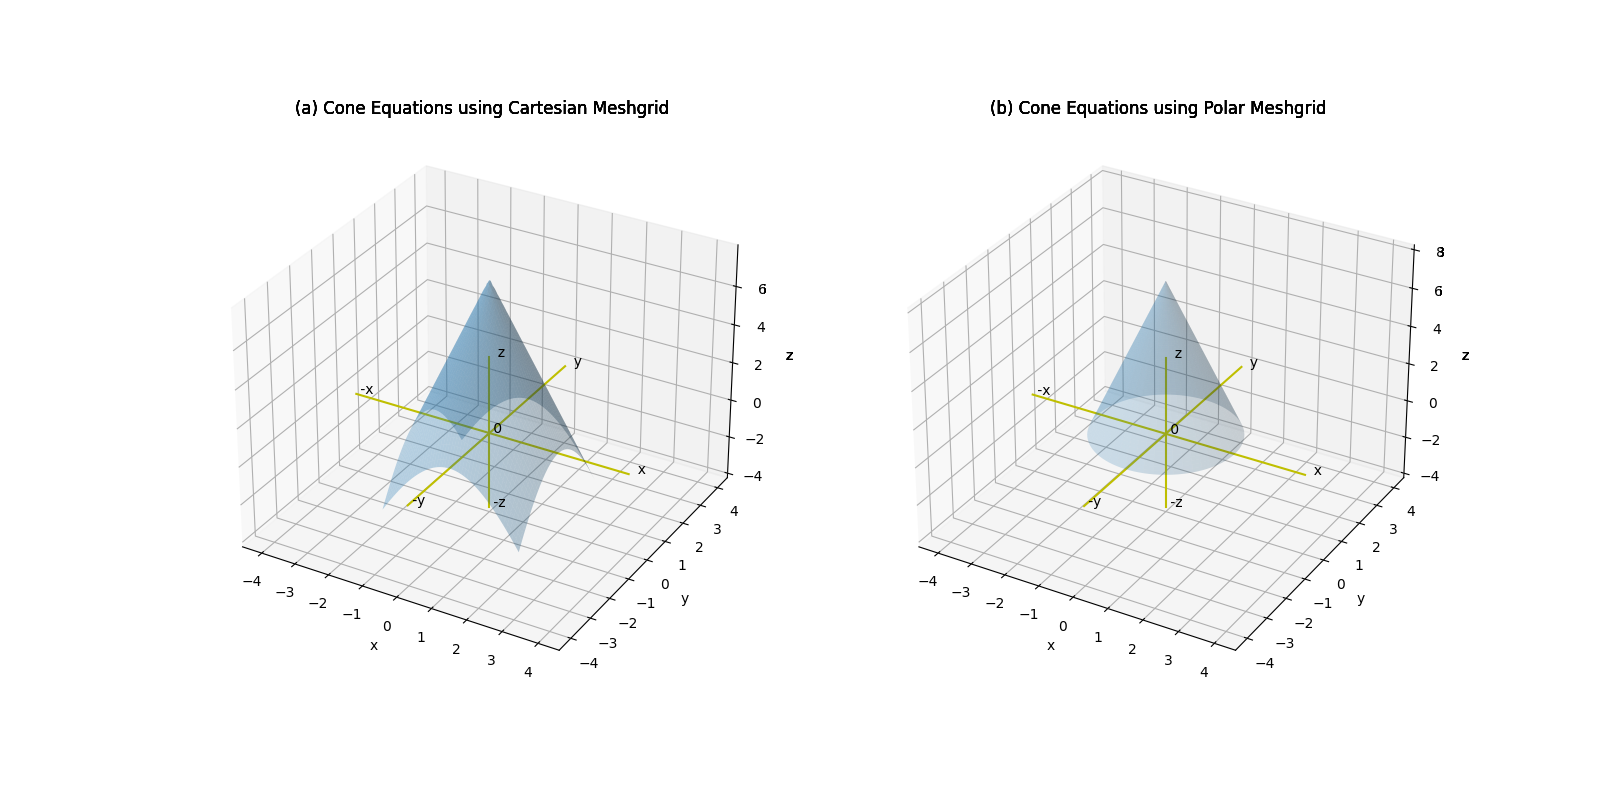
\includegraphics[width=1\linewidth,height=0.7\textheight]{Data/fgr01.png}
\caption{(a) Cone = f(x,y,z)  (b) Cone = f(rho,phi,z) }
\label{fig:Data/fgr01.png}
\end{figure}

\noindent Open Cone01.py. Study the codes and run the file.
 \par \ \par\noindent The equation in cylindrical coordinate systems is expressed as follows.
 \par \ \par\begin{equation}
 \begin{minipage}{250pt}
                \begin{flushleft} $\displaystyle \rho = \frac{b_{ase} \left(h_{eight} - z\right)}{h_{eight}}$  \end{flushleft}
 \end{minipage}
 \end{equation}
\noindent Note that $\phi$ is absent. It means that for any value of phi eConeCyl equation holds.
 \par \ \par\noindent The geometric relationship between Cartesian and cylindrical coordinate are expressed as follows.
 \par \ \par\begin{equation}
 \begin{minipage}{250pt}
                \begin{flushleft} $\displaystyle x = \rho \cos{\left(\phi \right)}$  \end{flushleft}
 \end{minipage}
 \end{equation}
\begin{equation}
 \begin{minipage}{250pt}
                \begin{flushleft} $\displaystyle y = \rho \sin{\left(\phi \right)}$  \end{flushleft}
 \end{minipage}
 \end{equation}
\begin{equation}
 \begin{minipage}{250pt}
                \begin{flushleft} $\displaystyle z = z$  \end{flushleft}
 \end{minipage}
 \end{equation}
\noindent The equation of cone can be found at \url{https://mathworld.wolfram.com/Cone.html} 
 \par \ \par\begin{equation}
 \begin{minipage}{250pt}
                \begin{flushleft} $\displaystyle \delta = 2 \operatorname{atan}{\left(\frac{b_{ase}}{h_{eight}} \right)}$  \end{flushleft}
 \end{minipage}
 \end{equation}
\begin{equation}
 \begin{minipage}{250pt}
                \begin{flushleft} $\displaystyle z = u$  \end{flushleft}
 \end{minipage}
 \end{equation}
\begin{equation}
 \begin{minipage}{250pt}
                \begin{flushleft} $\displaystyle x = \frac{b_{ase} \left(h_{eight} - u\right) \cos{\left(\phi \right)}}{h_{eight}}$  \end{flushleft}
 \end{minipage}
 \end{equation}
\begin{equation}
 \begin{minipage}{250pt}
                \begin{flushleft} $\displaystyle y = \frac{b_{ase} \left(h_{eight} - u\right) \sin{\left(\phi \right)}}{h_{eight}}$  \end{flushleft}
 \end{minipage}
 \end{equation}
\noindent The equations above is the converstion of cylindrical coordinate to cartesian systems.
 \par \ \par\begin{equation}
 \begin{minipage}{250pt}
                \begin{flushleft} $\displaystyle x = \frac{b_{ase} \left(h_{eight} - z\right) \cos{\left(\phi \right)}}{h_{eight}}$  \end{flushleft}
 \end{minipage}
 \end{equation}
\begin{equation}
 \begin{minipage}{250pt}
                \begin{flushleft} $\displaystyle y = \frac{b_{ase} \left(h_{eight} - z\right) \sin{\left(\phi \right)}}{h_{eight}}$  \end{flushleft}
 \end{minipage}
 \end{equation}
\begin{equation}
 \begin{minipage}{250pt}
                \begin{flushleft} $\displaystyle x = \frac{b_{ase} \left(h_{eight} - z\right) \cos{\left(\phi \right)}}{h_{eight}} = \rho \cos{\left(\phi \right)}$  \end{flushleft}
 \end{minipage}
 \end{equation}
\begin{equation}
 \begin{minipage}{250pt}
                \begin{flushleft} $\displaystyle y = \frac{b_{ase} \left(h_{eight} - z\right) \sin{\left(\phi \right)}}{h_{eight}} = \rho \sin{\left(\phi \right)}$  \end{flushleft}
 \end{minipage}
 \end{equation}
\noindent The symbolic math equation of a cone in Cartesian system is expressed as follows.
 \par \ \par\begin{equation}
 \begin{minipage}{250pt}
                \begin{flushleft} $\displaystyle x^{2} + y^{2} = \frac{b_{ase}^{2} \left(h_{eight} - z\right)^{2}}{h_{eight}^{2}}$  \end{flushleft}
 \end{minipage}
 \end{equation}
\noindent The base radius and height of the cone are given as follows.
 \par \ \par\begin{equation}
 \begin{minipage}{250pt}
                \begin{flushleft} $\displaystyle b_{ase} = 2$  \end{flushleft}
 \end{minipage}
 \end{equation}
\begin{equation}
 \begin{minipage}{250pt}
                \begin{flushleft} $\displaystyle h_{eight} = 8$  \end{flushleft}
 \end{minipage}
 \end{equation}
\noindent The equation of the cone is substituted with numerical parameters given above as follows.
 \par \ \par\begin{equation}
 \begin{minipage}{250pt}
                \begin{flushleft} $\displaystyle x^{2} + y^{2} = \frac{\left(z - 8\right)^{2}}{16}$  \end{flushleft}
 \end{minipage}
 \end{equation}
\noindent \section{Surface Plot Algorithms of a Cone }
 \par \ \par\noindent The mathematical expressions for surface plots in Cartesian coordinate system are expressed as follows.
 \par \ \par\begin{equation}
 \begin{minipage}{250pt}
                \begin{flushleft} $\displaystyle z = f{\left(x,y \right)}$  \quad where z is dependent variable and x and y are independent variables \end{flushleft}
 \end{minipage}
 \end{equation}
\begin{equation}
 \begin{minipage}{250pt}
                \begin{flushleft} $\displaystyle x = f{\left(z,y \right)}$  \quad where x is dependent variable and z and y are independent variables \end{flushleft}
 \end{minipage}
 \end{equation}
\begin{equation}
 \begin{minipage}{250pt}
                \begin{flushleft} $\displaystyle y = f{\left(x,z \right)}$  \quad where y is dependent variable and x and z are independent variables \end{flushleft}
 \end{minipage}
 \end{equation}
\noindent The mathematical expression for surface plots in cylindrical coordinate system are expressed as follos.
 \par \ \par\begin{equation}
 \begin{minipage}{250pt}
                \begin{flushleft} $\displaystyle \phi = f{\left(\rho,z \right)}$  \quad where phi is the dependent variable and rho and z are independent variables \end{flushleft}
 \end{minipage}
 \end{equation}
\begin{equation}
 \begin{minipage}{250pt}
                \begin{flushleft} $\displaystyle \rho = f{\left(\phi,z \right)}$  \quad where rho is the dependent variable and phi and z are independent variables \end{flushleft}
 \end{minipage}
 \end{equation}
\begin{equation}
 \begin{minipage}{250pt}
                \begin{flushleft} $\displaystyle z = f{\left(\phi,\rho \right)}$  \quad where z is the dependent variable and phi and rho are independent variables \end{flushleft}
 \end{minipage}
 \end{equation}
\noindent The surface plots of a cone in Figure 1 (a)  were generated by cone01.py codes. The dependent variable is z and the independent variables are x and y. Thus z = f(x,y). The algorithm of plot 1 is directly Cartesian meshgrid. Hence, mx,my = meshgrig(x,y). The meshgrid of z is mz=f(mx,my). 
 \par \ \par\noindent The algorithm of plot 2 is cylindrical meshgrid that is converted to Cartesian meshgrid. The surface equation in cylindrical coordinate system is $z = f{\left(\phi,\rho \right)}$.  Hence, cylindrical meshgrids is $m\phi,m\rho = meshgrid(\phi,\rho)$. Converting cylindrical meshgrids to Cartesian, $mx = m\rho cos(m\phi)$ and $my = m\rho sin(m\phi)$ by virtue of geometric relationship between Cartesian and Cylindrical coordinate systems. The meshgrid z is $mz=f(mx,my)$.
 \par \ \par\noindent \section{Intersection of a Cone and of a Plane }
 \par \ \par\noindent The equation of a cone in cylindrical system is expressed as follows.
 \par \ \par\begin{equation}
 \begin{minipage}{250pt}
                \begin{flushleft} $\displaystyle \rho = \frac{b_{ase} \left(h_{eight} - z\right)}{h_{eight}}$  \end{flushleft}
 \end{minipage}
 \end{equation}
\noindent The variable $\phi$ is absent. It means that for any value of $\phi$ the equation holds.
 \par \ \par\noindent To make the $\phi$ and $\rho$ as independent variables, the dependent varialble is z. Thus,
 \par \ \par\begin{equation}
 \begin{minipage}{250pt}
                \begin{flushleft} $\displaystyle z = \frac{h_{eight} \left(- \rho + b_{ase}\right)}{b_{ase}}$  \end{flushleft}
 \end{minipage}
 \end{equation}
\noindent The equations of a plane are expressed as follows.
 \par \ \par\begin{equation}
 \begin{minipage}{250pt}
                \begin{flushleft} $\displaystyle A x + B y + C z + K = 0$  \end{flushleft}
 \end{minipage}
 \end{equation}
\begin{equation}
 \begin{minipage}{250pt}
                \begin{flushleft} $\displaystyle z = f{\left(x,y \right)} = - \frac{2 x}{5} + \frac{8 y}{5} + 5$  \end{flushleft}
 \end{minipage}
 \end{equation}
\noindent The plot of a cone is shown in Figure 3.1 (a) and the plot of a plane is shown in Figure 3.1 (b).
 \par \ \par\begin{figure}[H]
\centering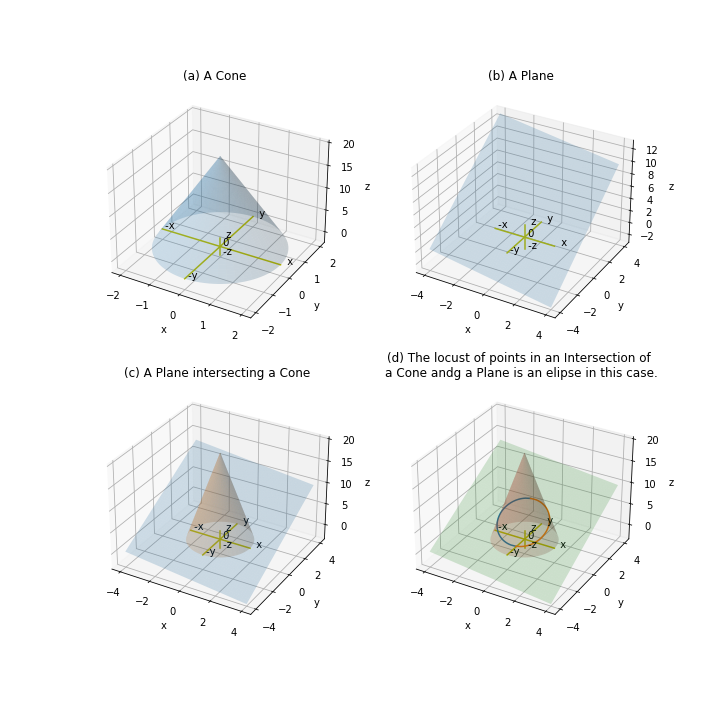
\includegraphics[width=1\linewidth,height=0.7\textheight]{Data/fgr02.png}
\caption{A plane overlapping with cone.}
\label{fig:Data/fgr02.png}
\end{figure}

\noindent The plot of the cone in Figure 3.1 (a) and the Plot of the plane in Figure 3.1 (b) were plotted together in Figure 3.1 (c). There exists locus of points that are common to both cone and plane surfaces. The locus of points defines a curve line. The curve line is an eliptical as shown in Figure 3.1 (d).
 \par \ \par\noindent The surface equations are expressed as z = f(x,y) or x=f(z,y) or y=f(x,z). The rhs has the independent variables. The lhs has the dependent variable. Consider the surface plots of a cone and a plane with z as the dependent variable and x and y as the independent variables. Thus,
 \par \ \par\begin{equation}
 \begin{minipage}{250pt}
                \begin{flushleft} $\displaystyle z_{c} = f{\left(x_{c},y_{c} \right)}$  \quad cone equation\end{flushleft}
 \end{minipage}
 \end{equation}
\begin{equation}
 \begin{minipage}{250pt}
                \begin{flushleft} $\displaystyle z_{p} = f{\left(x_{p},y_{p} \right)}$  \quad plane equation\end{flushleft}
 \end{minipage}
 \end{equation}
\noindent A line in 3D space where the cone and the plane intersected could be drawn and plotted. The locus of points must be the common points of the cone and the plane. Hence, x=xc=xp; y=yc=yp; and z=zc=zp
 \par \ \par\noindent The equations of the cone with xc a dependent variable and yc and zc as independent vatiable is expressed as follows.
 \par \ \par\begin{equation}
 \begin{minipage}{250pt}
                \begin{flushleft} $\displaystyle x_{c} = f{\left(y_{c},z_{c} \right)}$  \end{flushleft}
 \end{minipage}
 \end{equation}
\noindent The equations of the plane with yp a dependent variable and xp and zp as independent vatiable is expressed as follows.
 \par \ \par\begin{equation}
 \begin{minipage}{250pt}
                \begin{flushleft} $\displaystyle y_{p} = f{\left(x_{p},z_{p} \right)}$  \end{flushleft}
 \end{minipage}
 \end{equation}
\noindent Substituting yp in yc,
 \par \ \par\begin{equation}
 \begin{minipage}{250pt}
                \begin{flushleft} $\displaystyle x_{c} = f{\left(f{\left(x_{p},z_{p} \right)},z_{c} \right)}$  \end{flushleft}
 \end{minipage}
 \end{equation}
\noindent Since the locus of points of intersection must be the seame for both cone and plane, thus, 
 \par \ \par\begin{equation}
 \begin{minipage}{250pt}
                \begin{flushleft} $\displaystyle x = f{\left(f{\left(x,z \right)},z \right)}$  \end{flushleft}
 \end{minipage}
 \end{equation}
\noindent Solving for x,
 \par \ \par\begin{equation}
 \begin{minipage}{250pt}
                \begin{flushleft} $\displaystyle x = f{\left(z \right)}$  \end{flushleft}
 \end{minipage}
 \end{equation}
\noindent In like process,
 \par \ \par\begin{equation}
 \begin{minipage}{250pt}
                \begin{flushleft} $\displaystyle y = f{\left(z \right)}$  \end{flushleft}
 \end{minipage}
 \end{equation}
\noindent Given a set of values of z, the x and y are computed. The values of x, y, and z forms the locus of points common to both the cone and plane.
 \par \ \par\noindent The relationships of objects, equations and type of variables for plot algorithm are tabulated as follows.
 \par \ \par\noindent \begin{tabular}
{p{1cm} p{3cm} p{3cm} p{3cm} }
object& no of equations &no. of defendent variable &no. of independent variable \\ 
surface&1&1&2 \\ 
line&2&2&1 \\ 
point&0&0&3 \\ 
\end{tabular}
 \par \ \par\noindent \section{Conic Sections }
 \par \ \par\noindent The Figure 3 illustrate the mirrored cones that define conic section.
 \par \ \par\noindent The equation of upper cone expressed in terms Cartesian coordinate system is shown as follows.
 \par \ \par\begin{equation}
 \begin{minipage}{250pt}
                \begin{flushleft} $\displaystyle x^{2} + y^{2} = \frac{4 \left(z - 25\right)^{2}}{25}$  \end{flushleft}
 \end{minipage}
 \end{equation}
\noindent The equation of the disk in terms of Cartesian coordinate system is expressed as follows.
 \par \ \par\begin{equation}
 \begin{minipage}{250pt}
                \begin{flushleft} $\displaystyle z = 12$  \end{flushleft}
 \end{minipage}
 \end{equation}
\noindent The intersection of the upper cone with a disk is shown in Figure 3
 \par \ \par\noindent The disk plane intersecting with a cone generates a locus of points of     circle.
 \par \ \par\begin{figure}[H]
\centering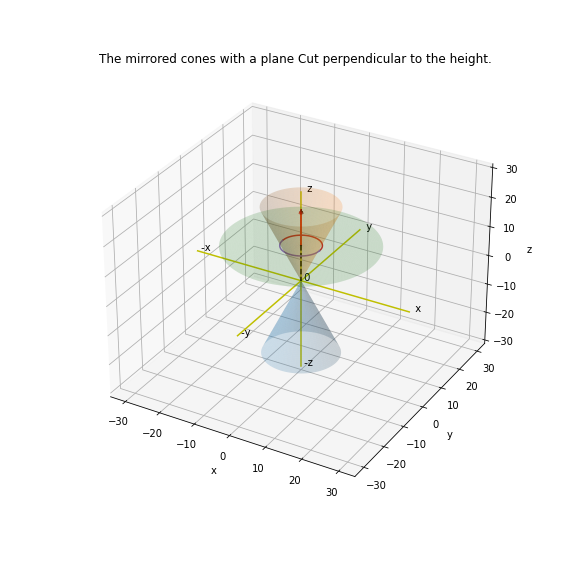
\includegraphics[width=1\linewidth,height=0.7\textheight]{Data/fgr03.png}
\caption{Cones section that defined a circle. }
\label{fig:Data/fgr03.png}
\end{figure}

\noindent The disk could be tilted and the locus of intersecting points forms an elipse.
 \par \ \par\noindent The equation of the tilted disk is expressed as follows.
 \par \ \par\begin{equation}
 \begin{minipage}{250pt}
                \begin{flushleft} $\displaystyle - 0.609710760849692 x + 0.7926239891046 z = 9.5114878692552$  \end{flushleft}
 \end{minipage}
 \end{equation}
\begin{figure}[H]
\centering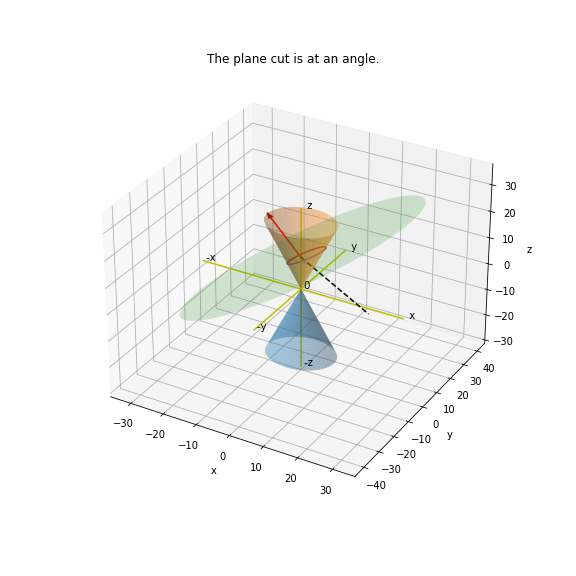
\includegraphics[width=1\linewidth,height=0.7\textheight]{Data/fgr04.png}
\caption{Conic section cut by disk plane at an angle genrated an elipse an eliptical locus of points.}
\label{fig:Data/fgr04.png}
\end{figure}

\noindent When the tilt is in parallel with the slope of the side of the cone, the    locus of points form a parabola.
 \par \ \par\noindent The equation of the disk tilted in parallel with the slope of the lateral side of the cone. The cone and the tilted disk is shown in Figure 5.
 \par \ \par\begin{equation}
 \begin{minipage}{250pt}
                \begin{flushleft} $\displaystyle - 0.970142500145332 y - 0.242535625036333 z = -7.76114000116266$  \end{flushleft}
 \end{minipage}
 \end{equation}
\begin{figure}[H]
\centering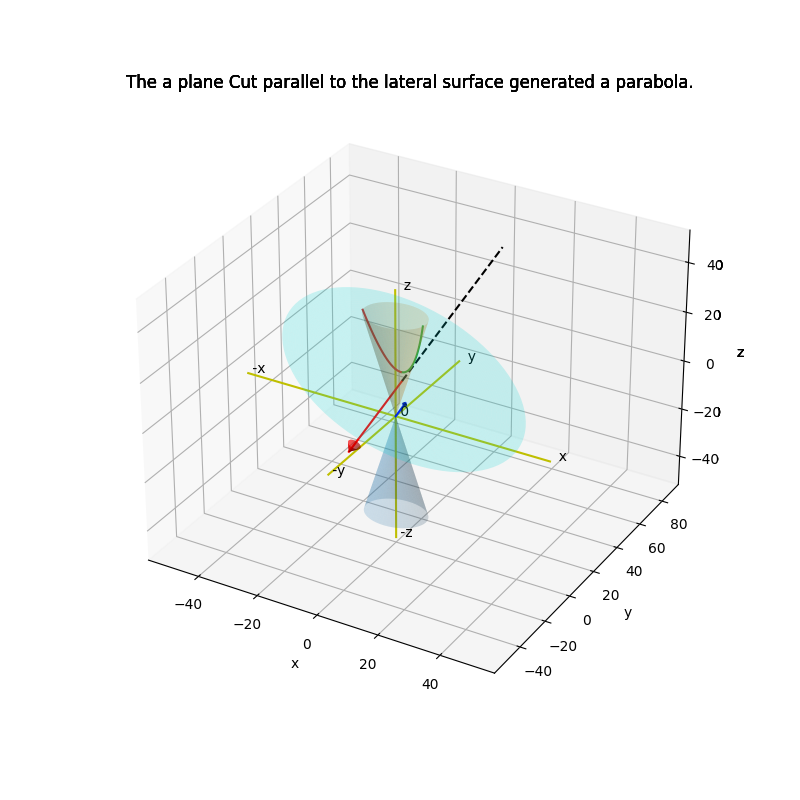
\includegraphics[width=1\linewidth,height=0.7\textheight]{Data/fgr05.png}
\caption{A Conic section that generated a parabola. }
\label{fig:Data/fgr05.png}
\end{figure}

\noindent When the disk plane is in parallel with the vertical axis of the cone,    the locus of points forms a hyperbola. Note the intersection cut across    both the upper and lower cones.
 \par \ \par\noindent The equation of the disk titled in parallel with the cone vertical axis is shown as follows.
 \par \ \par\begin{equation}
 \begin{minipage}{250pt}
                \begin{flushleft} $\displaystyle 1.0 y = 5.0$  \end{flushleft}
 \end{minipage}
 \end{equation}
\begin{figure}[H]
\centering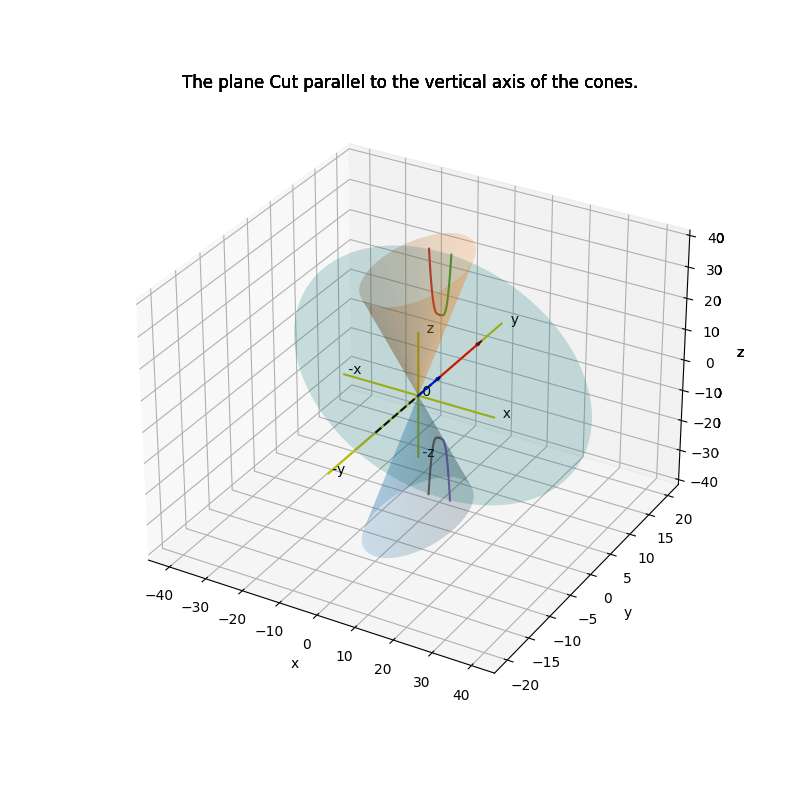
\includegraphics[width=1\linewidth,height=0.7\textheight]{Data/fgr06.png}
\caption{A Conic section that generated a hyperbola. }
\label{fig:Data/fgr06.png}
\end{figure}

\noindent \section{Exercises}
 \par \ \par\noindent 1. Create your own inverted and upright cones. The tips of the cones rest at origin. Formulate the cylindrical and Cartesian equations of the inverted and upright cones. (75)
 \par \ \par\noindent 2. Create your own plane disk perpendicular to the z axis and cut the upright cone below the origin. Choose your own distance value below the origin. Formulate the disk equation. (5) 
 \par \ \par\noindent 3. Formulate the two equations that define the locus of intersection points of the upright cone and the disk. (5)
 \par \ \par\noindent 4. What is the range of disk tilt angle such that the intersection forms circular and/or eliptical curve lines. (5) 
 \par \ \par\noindent 5. What is the disk angle of tilt such that the intersection forms a parabolic curve line. (5)
 \par \ \par\noindent 6. What is the disk angle of tilt such that the intersection forms a hyperbolic curve lines. (5)
 \par \ \par\noindent \nocite{2}
 \par \ \par\noindent \nocite{3}
 \par \ \par\noindent \nocite{7}
 \par \ \par\noindent \nocite{8}
 \par \ \par\noindent \nocite{9}
 \par \ \par\noindent \nocite{11}
 \par \ \par\noindent \nocite{13}
 \par \ \par\noindent \nocite{15}
 \par \ \par\noindent \nocite{202}
 \par \ \par\noindent \nocite{203}
 \par \ \par\noindent \bibliographystyle{plain} 
 \bibliography{ccoLib/ccobib}
 \par \ \par\noindent \end{CJK*}
 \par \ \par\end{document}